\section{Experiments}
\label{sec:results}

We evaluated HTCL on (i) three image classification benchmarks: SplitMNIST~\cite{lecun2002gradient} (10 classes divided into 5 tasks, 2 classes per task), Split CIFAR-100~\cite{krizhevsky2009learning} (100 classes divided into 10 tasks, 10 classes per task) and a 100-class subset of ImageNet~\cite{deng2009imagenet} (ImageNet-100, 10 tasks of 10 classes each); (ii) a graph node classification problem using the Split Cora dataset~\cite{mccallum2000automating}; and (iii) a text classification problem on 20 Newsgroups~\cite{lang1995newsweeder} dataset  to demonstrate HTCL's generality across domains. All experiments other than ImageNet-100 use the \textit{domain-incremental} learning setting. ImageNet-100 is evaluated under both \textit{domain-incremental} and \textit{class-incremental} protocols (see Appendix~\ref{app:large-scale}). All experiments are performed on an NVIDIA A100 GPU.

\begin{figure*}[!htbp]
    \centering
    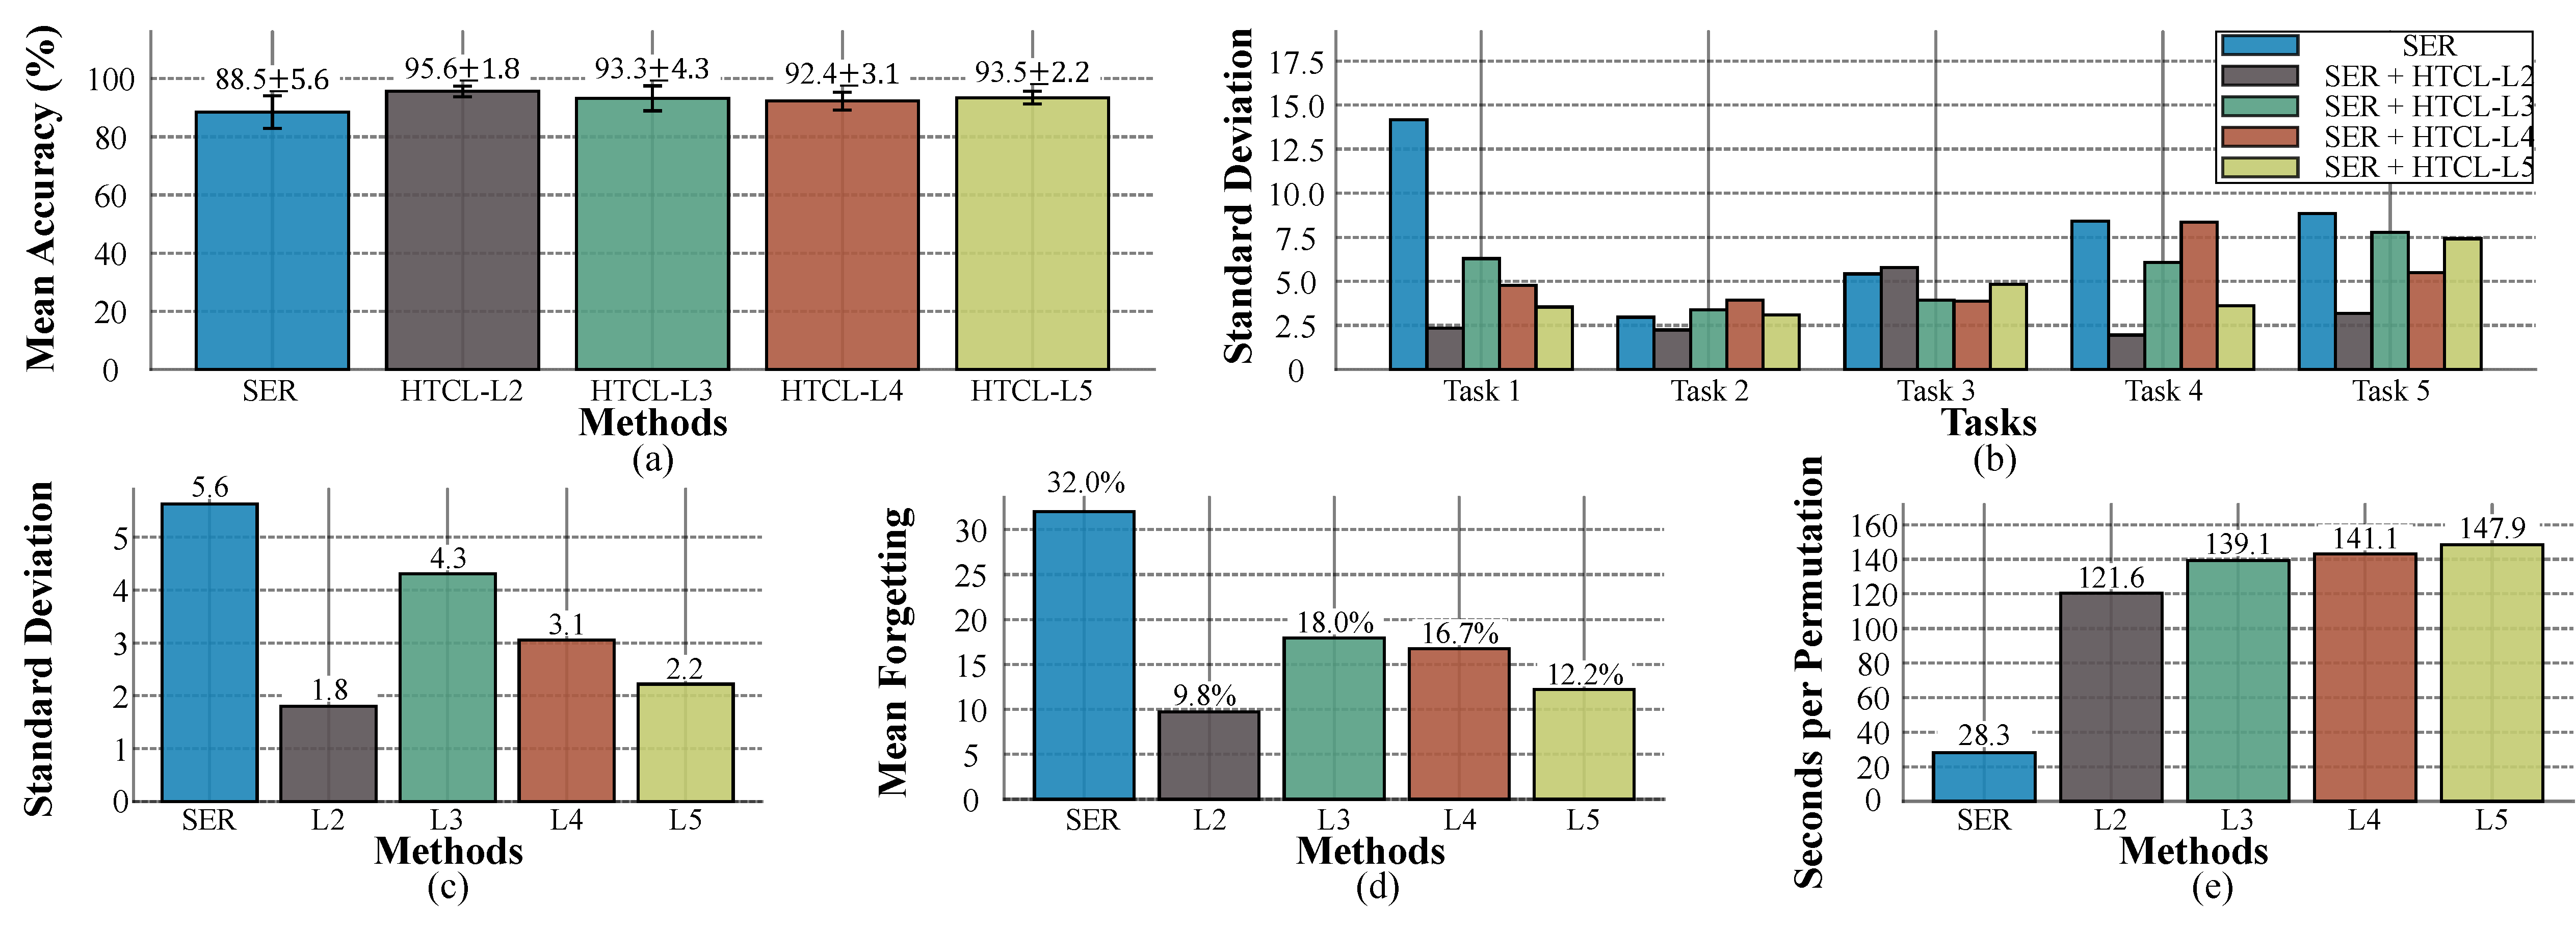
\includegraphics[width=0.90\textwidth, trim={0.3cm 0.3cm 0.3cm 0.3cm}, clip]{figures/updated_figures/ser.pdf}
    \caption{\textbf{Task-order robustness and memory retention of HTCL with SER on SplitMNIST.} 
    (a) Mean accuracy with standard-deviation error bars for SER and SER + HTCL-L\{2,3,4,5\}. 
    (b) Per-task standard deviation across permutations. 
    (c) Overall standard deviation. 
    (d) Mean forgetting. 
    (e) Wall-clock time per permutation. 
    HTCL reduces task-order variance and forgetting at moderate compute overhead.}
    \label{fig:ser-results}
\end{figure*}

\begin{figure}[!t]
  \centering
  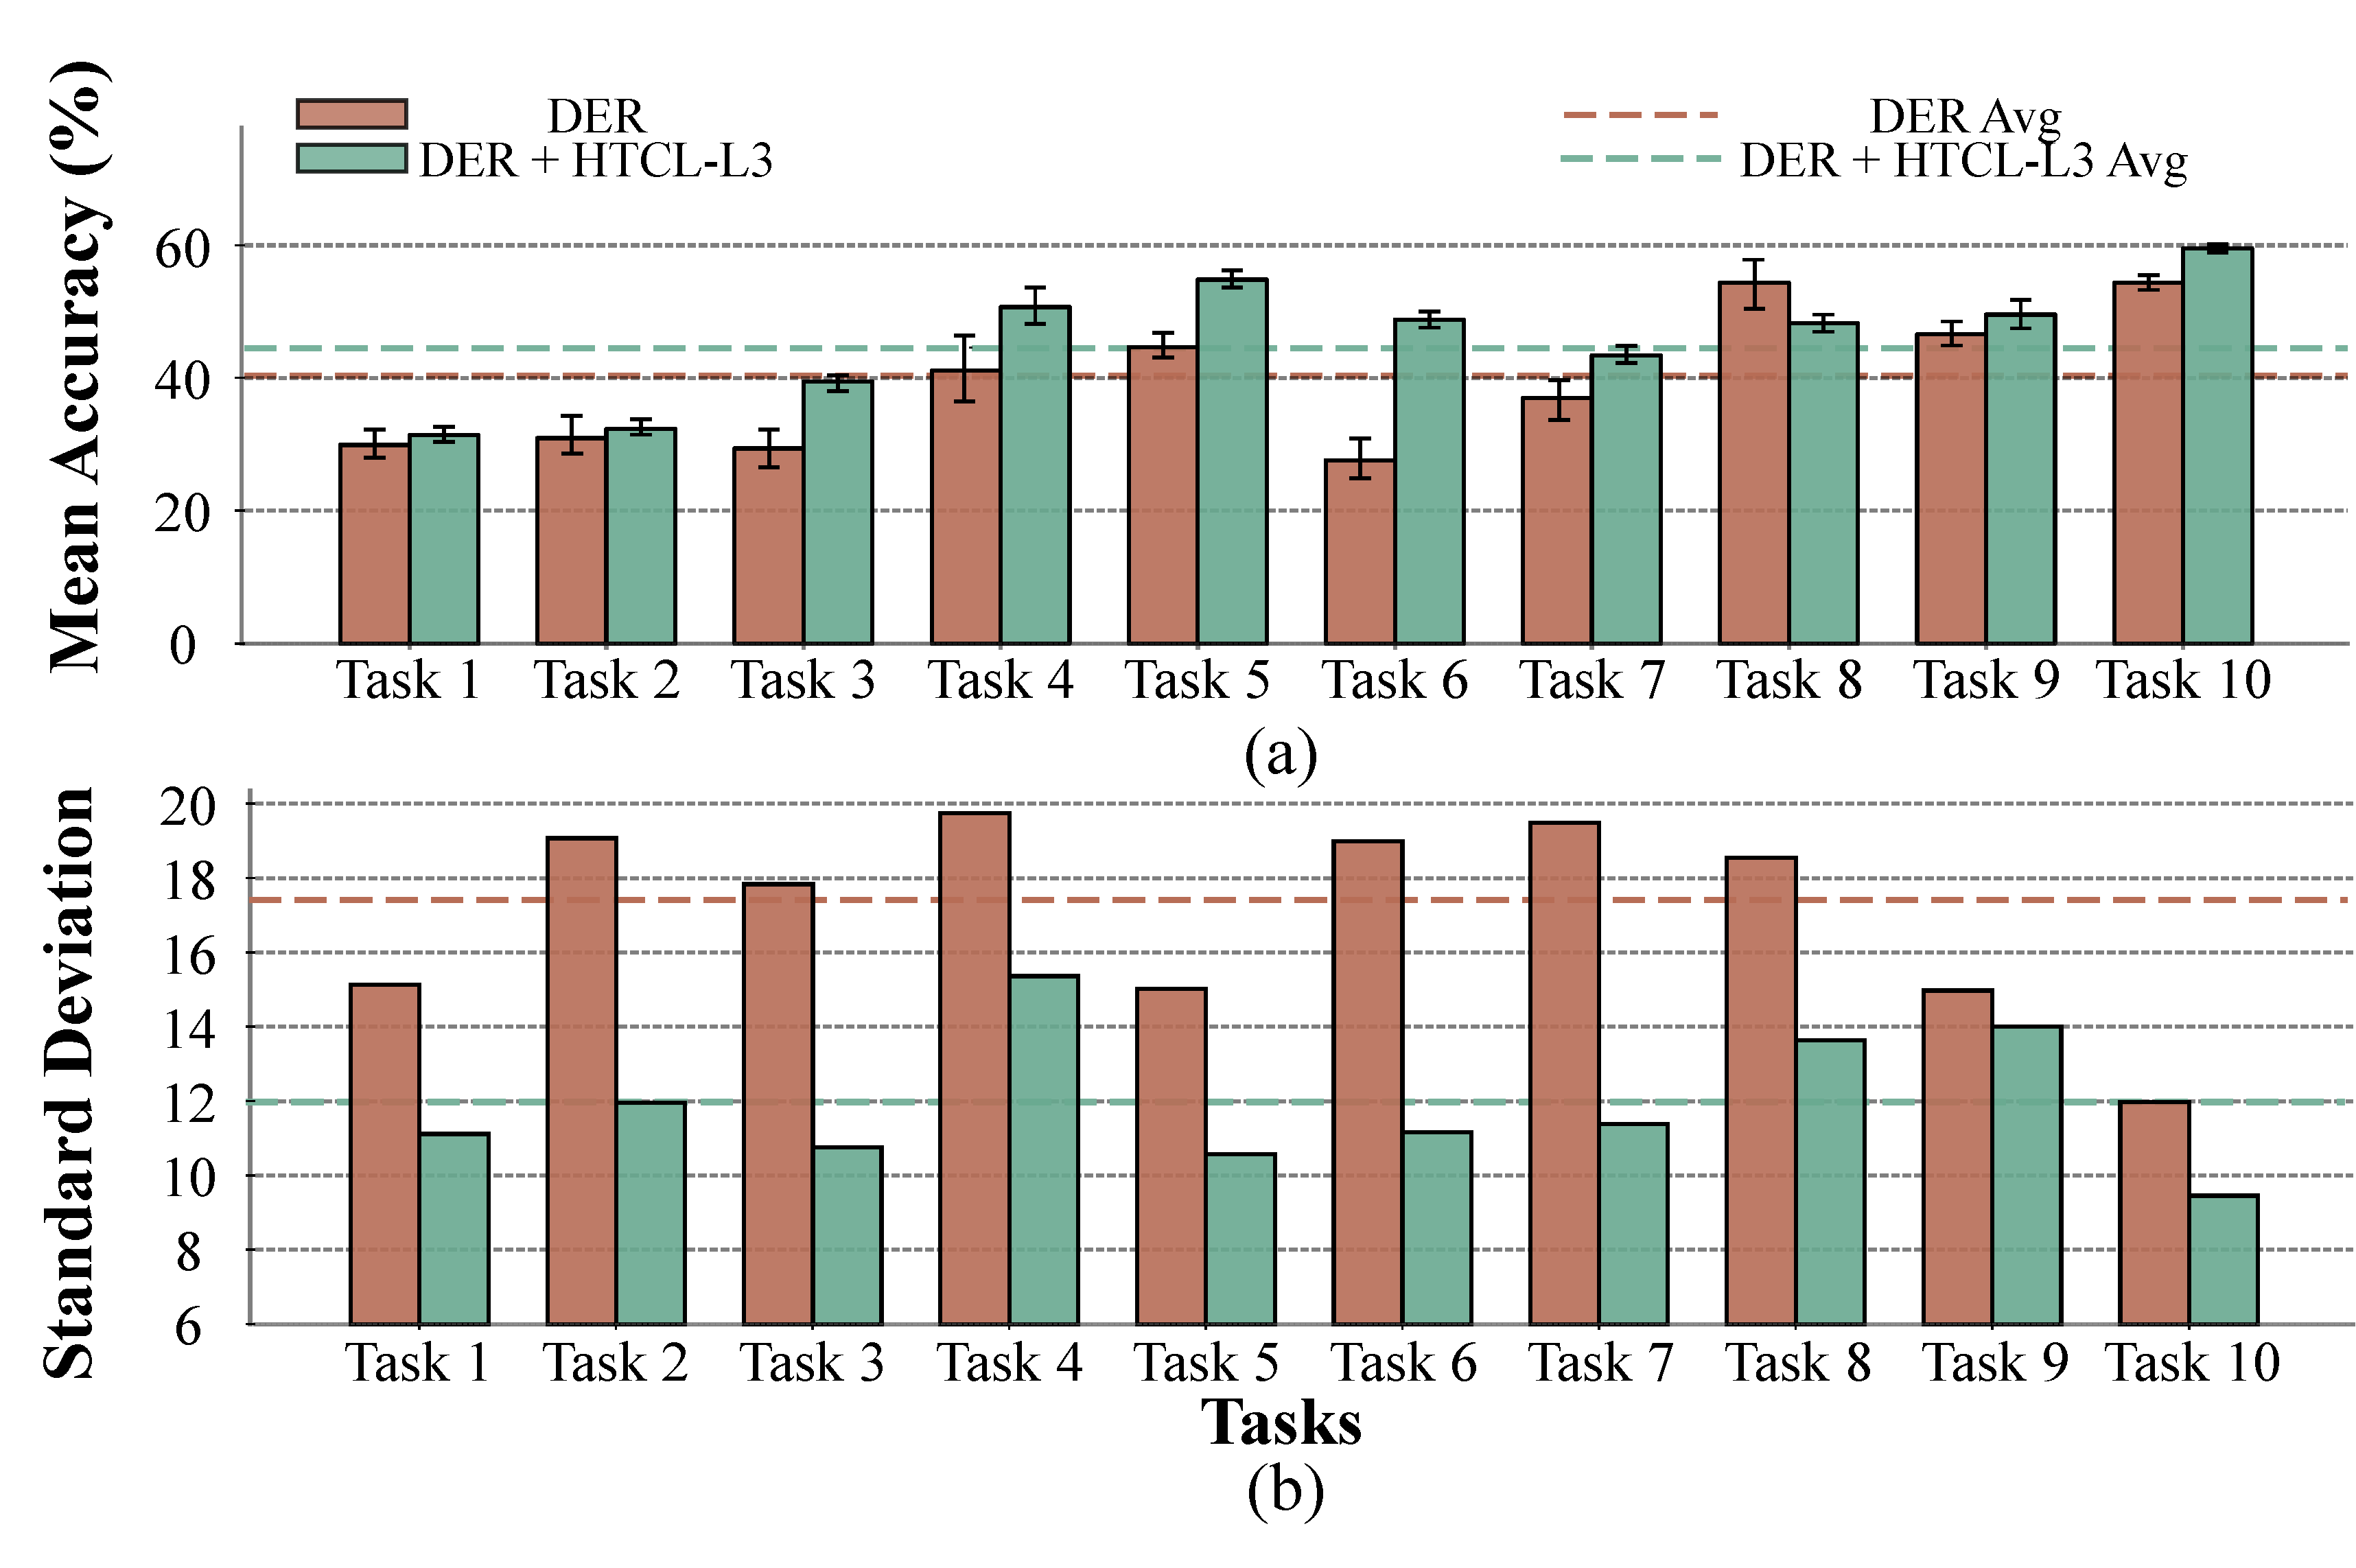
\includegraphics[width=\columnwidth]{figures/updated_figures/der.pdf}
  \caption{\textbf{Scalability of HTCL under long task sequences.} We extend the two-level local–global structure to a three-level hierarchy as described in Eq.~\eqref{eq:multi_hierarchy}, using DER as a baseline for illustration. The three-layer HTCL demonstrates higher memory retention and lower variance when handling long task sequences. (a) Mean accuracy per task: DER + HTCL-L3 achieves $45.2\%$ compared to $40.6\%$ for DER alone. (b) Standard deviation per task: DER + HTCL-L3 maintains a lower standard deviation ($12.0$) compared to DER alone ($17.4$).}
    \label{fig:extended}
\end{figure}

We compared the HTCL method against top seven baseline CL methods spanning replay-based, regularization-based, and hybrid approaches: Strong Experience Replay (SER)~\cite{zhuo2023continual}, Dark Experience Replay (DER)~\cite{buzzega2020dark}, Experience Replay (ER), DualNet~\cite{pham2021dualnet}, iCaRL~\cite{rebuffi2017icarl}, EWC~\cite{kirkpatrick2017overcoming}, and Spectral Regularizer (SR)~\cite{ICLR2025_5565ab68}. These baselines were selected to include methods with state-of-the-art performance on our benchmarks (SER), foundational approaches in CL (EWC, ER), and recently proposed techniques (SR). In our framework, each baseline trains the \textit{local} model, while the consolidated model is updated via the Taylor series–based rule in Eq.~\eqref{eq:hier_update-main}. We calculate \textit{average accuracy}, \textit{average forgetting} and \textit{standard deviation} of accuracy to demonstrate our results~\cite{lopez2017gradient, chaudhry2018efficient}. A detailed list of hyperparameters and other details on experimental setup can be found in Appendix~\ref{app:extended-results}.

We first present representative results illustrating the performance of HTCL on SplitMNIST (see Figure~\ref{fig:ser-results}) using SER as a baseline through mean accuracy, task-order sensitivity, forgetting, and computational overhead. Next, we demonstrate the scalability of our HTCL to extended task sequences using DER on Split CIFAR-100 (see Figure~\ref{fig:extended}). A comprehensive comparison against seven baseline models across four diverse datasets (SplitMNIST, Split CIFAR-100, Split Cora, 20 Newsgroups) can be found in Table~\ref{tab:mean-std}. We further investigate the effects of memory buffer size on HTCL performance in Appendix~\ref{app:small-buffer}. Finally, since our consolidation method resembles some similarities with federated aggregation, we present a comparative analysis against FedProx~\cite{li2020federated} and FedAvg~\cite{mcmahan2017communication} in Appendix~\ref{app:federated}.

\textbf{Enhanced task-order robustness.} Panels~(b) and~(c)  of Figure~\ref{fig:ser-results} characterize stability with respect to task-order permutations. Panel~(b) shows that HTCL enables lower per-task variance, with reductions of up to $82\%$ on the most volatile tasks (e.g., Task 1), suggesting that individual tasks are less sensitive to the order in which they are encountered. Panel~(c) summarizes this effect at the sequence level, where HTCL markedly reduces the overall standard deviation by $67.9\%$ (dropping from $5.6$ to $1.8$) across permutations, with HTCL-L2 exhibiting the strongest robustness. This stabilizing effect generalizes effectively to other modalities; on Cora (graph) and 20 Newsgroups (text), HTCL reduces standard deviation by approximately $38\%$ and $33\%$ respectively, confirming that the method's robustness is not limited to image domains (results are shown in Table~\ref{tab:mean-std}).

\textbf{Accuracy and memory retention.} Panel~(a) in Figure~\ref{fig:ser-results} shows that incorporating the Taylor-based consolidation consistently improves mean accuracy relative to the SER baseline, with HTCL-L2 achieving the largest gain of $7.1$ percentage points ($95.6\%$ vs $88.5\%$). We observe similar improvements in non-image tasks, where HTCL boosts mean accuracy by $5.8$ percentage points on Cora and $6.3$ percentage points on 20 Newsgroups. This improvement reflects stronger retention of earlier tasks rather than overfitting to the final task, a trend that is corroborated by the forgetting metric in Panel~(d), where HTCL-L2 exhibits a drastic drop in forgetting compared to the baseline ($9.8\%$ vs $32.0\%$). This $22.2\%$ reduction on SplitMNIST is mirrored in the graph and text domains, where forgetting drops by over $10$ percentage points relative to the baseline. These results indicate that the global consolidation step effectively preserves previously learned representations, preventing the catastrophic overwriting of weights associated with earlier tasks. Together, these results demonstrate that the observed accuracy gains stem principally from improved long-term memory retention.

\begin{figure*}[!t]
    \centering
    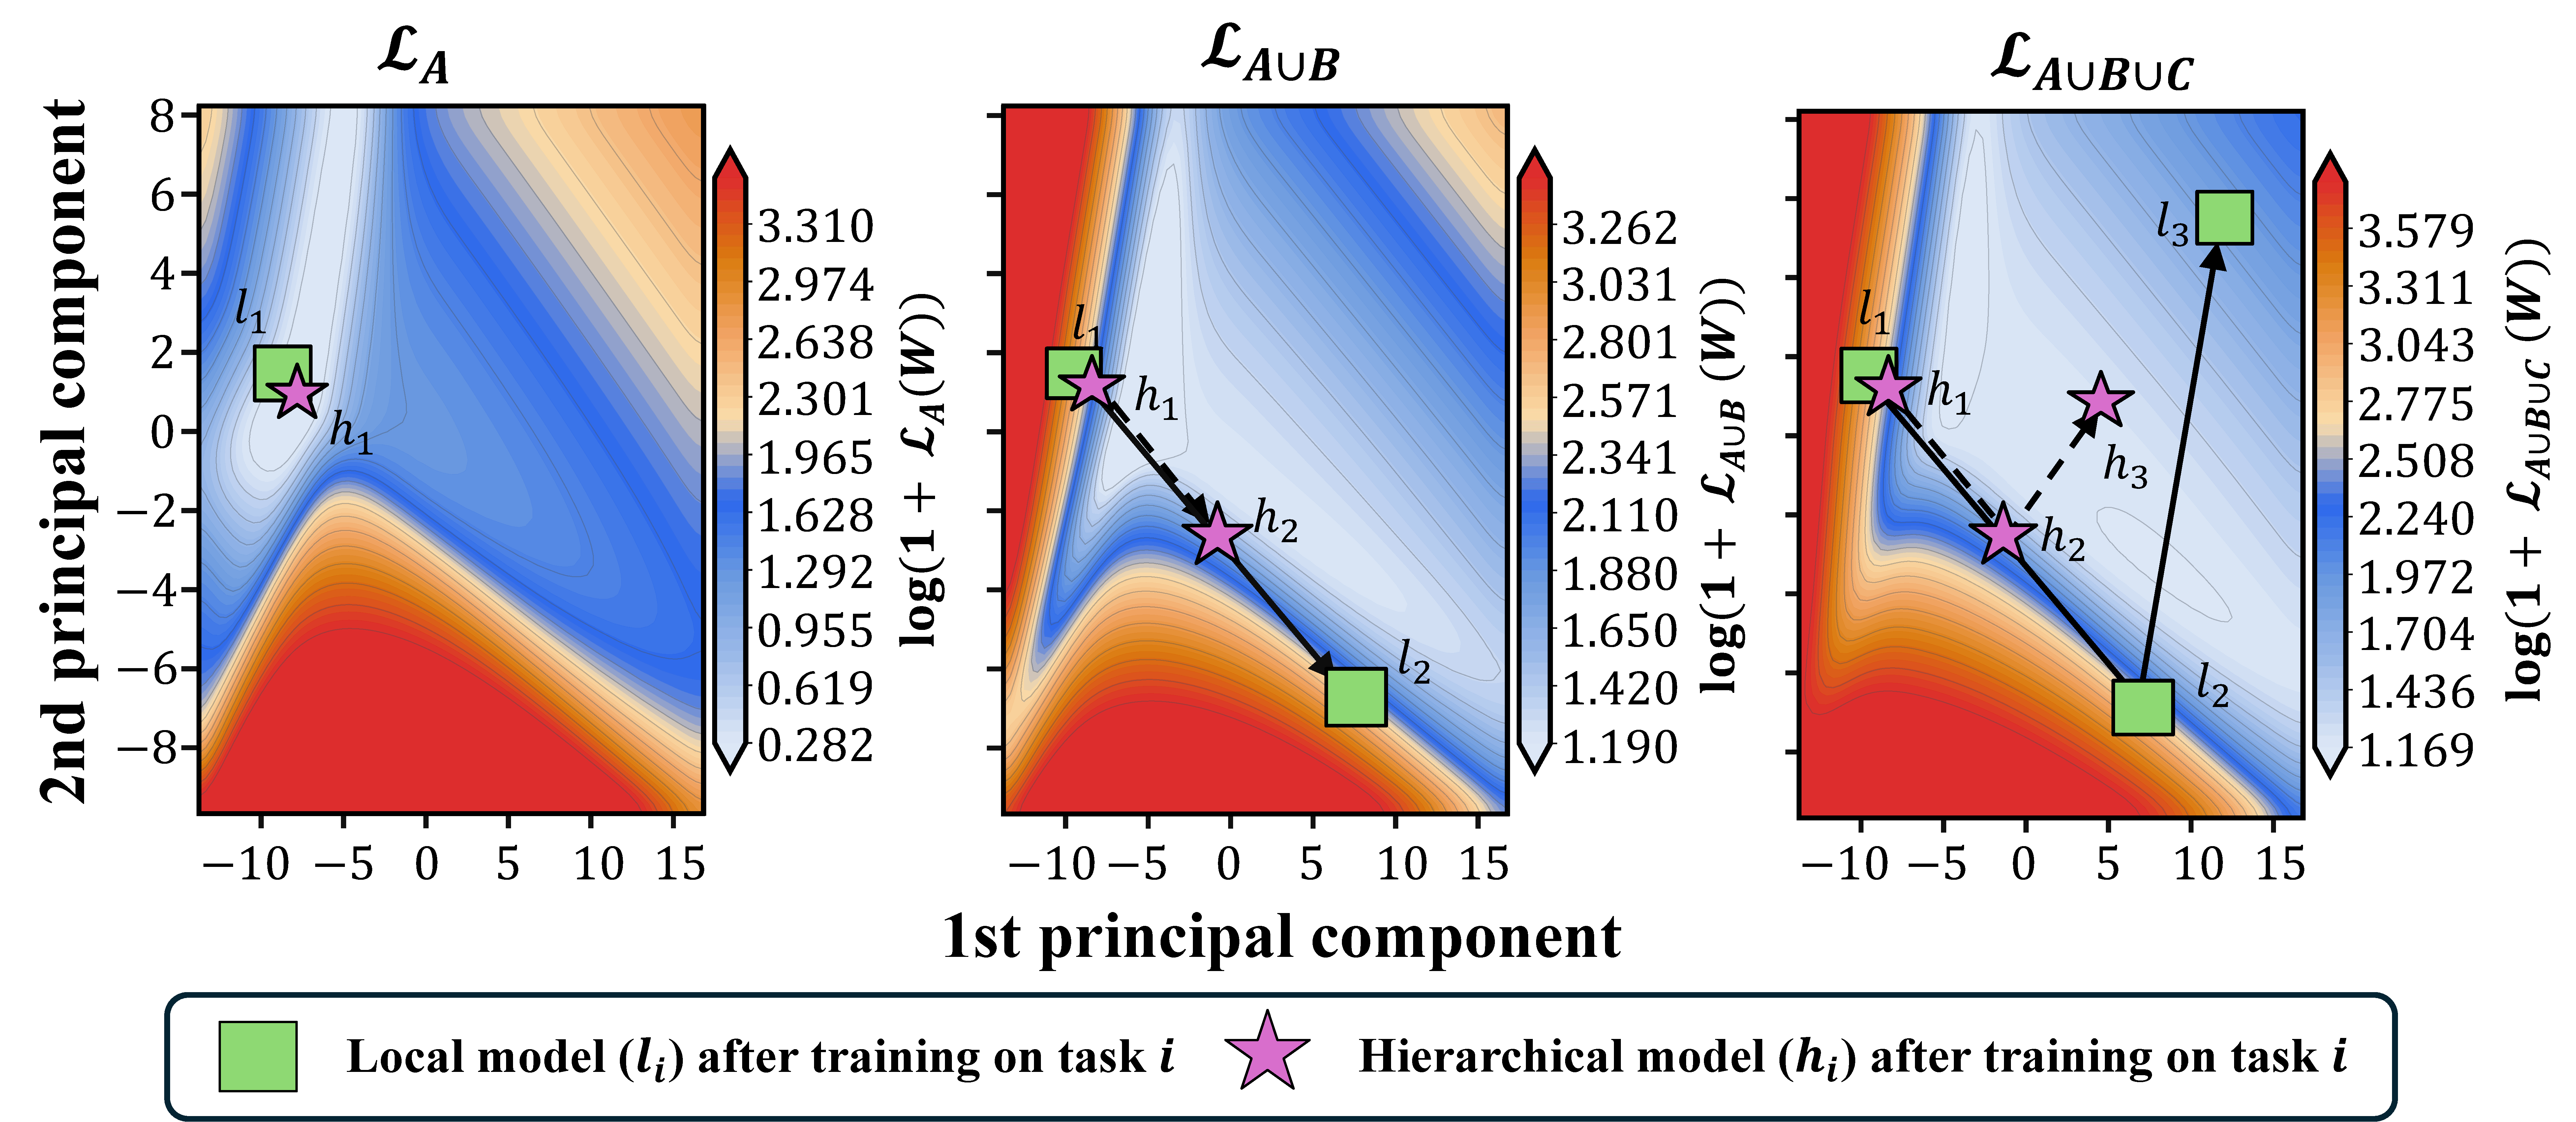
\includegraphics[width=0.8\textwidth]{figures/loss_landscape/loss_landscape.pdf}
    \caption{\textbf{Loss-landscape geometry of HTCL across a SplitMNIST class-incremental sequence.} Green squares mark local models $\ell_i$ adapted to task $i$; pink stars mark hierarchical models $h_i$ after Taylor consolidation. Across panels, the local trajectory drifts toward task-specific minima along ridges of the cumulative loss, while the hierarchical trajectory remains within the shared low-loss corridor of $\mathcal{L}_{A \cup B \cup C}$.}
    \label{fig:loss_landscape}
\end{figure*}

\begin{table*}[!htbp]
\centering
\caption{Final accuracy and variability across domains under the domain-incremental setting using a replay buffer of 50 samples for SplitMNIST, Cora, and 20 Newsgroups, and 500 samples for CIFAR-100. Mean accuracy, standard deviation, and mean forgetting are computed over 120 task-order permutations for SplitMNIST and 20 Newsgroups, 6 permutations for Cora, and 200 random permutations for CIFAR-100. Across all methods, incorporating HTCL consistently reduces task-order sensitivity, yielding substantially lower standard deviations while preserving or improving mean accuracy. $\uparrow$ denotes an increase and $\downarrow$ denotes a decrease relative to the baseline. Best results within each method group are shown in \textbf{bold}.}
\label{tab:mean-std}
\resizebox{\textwidth}{!}{%
\begin{tabular}{lcccccccccccc}
\hline
\multirow{2}{*}{\textbf{Method}} &
  \multicolumn{12}{c}{\textbf{Datasets}} \\ \cline{2-13} 
 &
  \multicolumn{3}{c}{\textbf{SplitMNIST}} &
  \multicolumn{3}{c}{\textbf{CIFAR-100}} & 
  \multicolumn{3}{c}{\textbf{Cora}} & 
  \multicolumn{3}{c}{\textbf{20 Newsgroups}} \\ \hline
 &
  \textbf{Mean Acc.} &
  \textbf{Std} &
  \textbf{Mean Forget} &
  \textbf{Mean Acc.} &
  \textbf{Std} &
  \textbf{Mean Forget} &
  \textbf{Mean Acc.} &
  \textbf{Std} &
  \textbf{Mean Forget} &
  \textbf{Mean Acc.} &
  \textbf{Std} &
  \textbf{Mean Forget} \\ \hline
SER &
  88.5 & 5.6 & 32.0 &
  42.6 & 18.7 & 56.5 &
  72.5 & 6.8 & 28.5 &
  58.2 & 8.4 & 35.2 \\
SER + HTCL-L2 &
  \textbf{95.6}$\uparrow$ & \textbf{1.8}$\downarrow$ & \textbf{9.8}$\downarrow$ &
  44.7$\uparrow$ & 14.9$\downarrow$ & 40.0$\downarrow$ &
  \textbf{78.3}$\uparrow$ & \textbf{4.2}$\downarrow$ & \textbf{18.2}$\downarrow$ &
  \textbf{64.5}$\uparrow$ & \textbf{5.6}$\downarrow$ & \textbf{24.8}$\downarrow$ \\
SER + HTCL-L3 &
  93.3$\uparrow$ & 4.3$\downarrow$ & 18.0$\downarrow$ &
  \textbf{46.2}$\uparrow$ & \textbf{12.5}$\downarrow$ & \textbf{30.0}$\downarrow$ &
  76.8$\uparrow$ & 5.1$\downarrow$ & 21.4$\downarrow$ &
  62.8$\uparrow$ & 6.3$\downarrow$ & 27.5$\downarrow$ \\ \hline
DER &
  86.5 & 4.9 & 35.0 &
  40.6 & 17.4 & 58.2 &
  70.2 & 7.2 & 30.8 &
  55.8 & 9.1 & 38.4 \\
DER + HTCL-L2 &
  \textbf{95.1}$\uparrow$ & \textbf{1.8}$\downarrow$ & \textbf{10.2}$\downarrow$ &
  43.0$\uparrow$ & 14.4$\downarrow$ & 42.6$\downarrow$ &
  \textbf{77.5}$\uparrow$ & \textbf{4.5}$\downarrow$ & \textbf{19.5}$\downarrow$ &
  \textbf{62.3}$\uparrow$ & \textbf{6.0}$\downarrow$ & \textbf{26.5}$\downarrow$ \\
DER + HTCL-L3 &
  92.3$\uparrow$ & 4.3$\downarrow$ & 18.8$\downarrow$ &
  \textbf{45.2}$\uparrow$ & \textbf{12.0}$\downarrow$ & \textbf{33.0}$\downarrow$ &
  75.2$\uparrow$ & 5.4$\downarrow$ & 22.8$\downarrow$ &
  60.5$\uparrow$ & 6.8$\downarrow$ & 29.2$\downarrow$ \\ \hline
ER &
  89.3 & 5.5 & 30.3 &
  38.0 & 20.0 & 60.0 &
  68.5 & 7.8 & 32.5 &
  54.4 & 9.8 & 42.0 \\
ER + HTCL-L2 &
  \textbf{92.0}$\uparrow$ & \textbf{3.5}$\downarrow$ & \textbf{12.5}$\downarrow$ &
  41.0$\uparrow$ & 17.0$\downarrow$ & 48.0$\downarrow$ &
  \textbf{74.2}$\uparrow$ & \textbf{5.2}$\downarrow$ & \textbf{22.0}$\downarrow$ &
  \textbf{58.5}$\uparrow$ & \textbf{6.8}$\downarrow$ & \textbf{32.5}$\downarrow$ \\
ER + HTCL-L3 &
  91.5$\uparrow$ & 4.0$\downarrow$ & 14.0$\downarrow$ &
  \textbf{43.5}$\uparrow$ & \textbf{15.5}$\downarrow$ & \textbf{40.0}$\downarrow$ &
  73.0$\uparrow$ & 5.8$\downarrow$ & 24.5$\downarrow$ &
  57.2$\uparrow$ & 7.4$\downarrow$ & 34.0$\downarrow$ \\ \hline
iCaRL &
  93.2 & 4.8 & 12.5 &
  41.8 & 17.2 & 54.4 &
  74.8 & 6.2 & 22.5 &
  60.5 & 7.5 & 30.2 \\
iCaRL + HTCL-L2 &
  \textbf{96.1}$\uparrow$ & \textbf{2.1}$\downarrow$ & \textbf{6.8}$\downarrow$ &
  44.2$\uparrow$ & 14.0$\downarrow$ & 42.5$\downarrow$ &
  \textbf{78.2}$\uparrow$ & \textbf{3.8}$\downarrow$ & \textbf{15.8}$\downarrow$ &
  \textbf{65.8}$\uparrow$ & \textbf{5.0}$\downarrow$ & \textbf{22.5}$\downarrow$ \\
iCaRL + HTCL-L3 &
  95.0$\uparrow$ & 3.4$\downarrow$ & 9.2$\downarrow$ &
  \textbf{46.6}$\uparrow$ & \textbf{11.8}$\downarrow$ & \textbf{35.0}$\downarrow$ &
  77.5$\uparrow$ & 4.5$\downarrow$ & 18.2$\downarrow$ &
  64.0$\uparrow$ & 5.8$\downarrow$ & 25.0$\downarrow$ \\ \hline
DualNet &
  89.2 & 9.0 & 15.0 &
  40.6 & 17.5 & 57.0 &
  71.8 & 8.5 & 26.2 &
  56.5 & 10.2 & 33.5 \\
DualNet + HTCL-L2 &
  90.5$\uparrow$ & 6.0$\downarrow$ & 10.5$\downarrow$ &
  41.5$\uparrow$ & 14.4$\downarrow$ & 45.0$\downarrow$ &
  75.5$\uparrow$ & 5.8$\downarrow$ & 19.0$\downarrow$ &
  61.2$\uparrow$ & 7.2$\downarrow$ & 26.8$\downarrow$ \\
DualNet + HTCL-L3 &
  \textbf{91.0}$\uparrow$ & \textbf{5.5}$\downarrow$ & \textbf{9.0}$\downarrow$ &
  \textbf{44.0}$\uparrow$ & \textbf{12.0}$\downarrow$ & \textbf{36.0}$\downarrow$ &
  \textbf{76.8}$\uparrow$ & \textbf{5.2}$\downarrow$ & \textbf{17.5}$\downarrow$ &
  \textbf{62.5}$\uparrow$ & \textbf{6.5}$\downarrow$ & \textbf{24.5}$\downarrow$ \\ \hline
SR &
  88.0 & 7.5 & 31.0 &
  13.0 & 24.0 & 65.0 &
  69.5 & 8.8 & 35.0 &
  54.2 & 10.5 & 40.5 \\
SR + HTCL-L2 &
  90.0$\uparrow$ & 5.0$\downarrow$ & 14.0$\downarrow$ &
  18.5$\uparrow$ & 20.0$\downarrow$ & 55.0$\downarrow$ &
  74.0$\uparrow$ & 6.0$\downarrow$ & 25.5$\downarrow$ &
  59.6$\uparrow$ & 7.5$\downarrow$ & 32.7$\downarrow$ \\
SR + HTCL-L3 &
  \textbf{91.0}$\uparrow$ & \textbf{4.0}$\downarrow$ & \textbf{12.0}$\downarrow$ &
  \textbf{22.0}$\uparrow$ & \textbf{18.0}$\downarrow$ & \textbf{48.0}$\downarrow$ &
  \textbf{75.5}$\uparrow$ & \textbf{5.2}$\downarrow$ & \textbf{22.0}$\downarrow$ &
  \textbf{61.0}$\uparrow$ & \textbf{6.8}$\downarrow$ & \textbf{29.1}$\downarrow$ \\ \hline
EWC &
  79.3 & 9.8 & 42.8 &
  12.5 & 23.5 & 68.0 &
  65.2 & 9.7 & 38.2 &
  48.5 & 11.1 & 45.8 \\
EWC + HTCL-L2 &
  85.2$\uparrow$ & 6.2$\downarrow$ & 28.9$\downarrow$ &
  16.8$\uparrow$ & 19.5$\downarrow$ & 58.0$\downarrow$ &
  70.9$\uparrow$ & 6.5$\downarrow$ & 28.6$\downarrow$ &
  54.7$\uparrow$ & 8.8$\downarrow$ & 35.5$\downarrow$ \\
EWC + HTCL-L3 &
  \textbf{87.0}$\uparrow$ & \textbf{5.0}$\downarrow$ & \textbf{24.0}$\downarrow$ &
  \textbf{19.3}$\uparrow$ & \textbf{17.1}$\downarrow$ & \textbf{52.5}$\downarrow$ &
  \textbf{72.5}$\uparrow$ & \textbf{5.8}$\downarrow$ & \textbf{25.5}$\downarrow$ &
  \textbf{56.0}$\uparrow$ & \textbf{7.2}$\downarrow$ & \textbf{33.3}$\downarrow$ \\ \hline
\end{tabular}%
}
\end{table*}

\textbf{Practical computational overhead.} Panel~(e) reports the computation time per permutation. HTCL introduces additional cost, increasing the time per permutation from $28.3$ seconds (SER) to $121.6$ seconds (HTCL-L2). However, this overhead scales gradually with hierarchy depth. In practice, this trade-off is highly favorable: while computational cost increases by approximately $4\times$, it yields a $69\%$ relative reduction in forgetting ($32.0\%$ to $9.8\%$) and a $68\%$ reduction in task-order variance ($5.6$ to $1.8$). This makes the method practical for CL scenarios where reliability and robustness to random task order are priorities over raw training speed.

\textbf{Generalization across methods.} Table~\ref{tab:mean-std} reports mean accuracy, standard deviation, and mean forgetting across multiple CL baselines under the domain-incremental setting. Across all baseline methods, incorporating HTCL consistently reduces standard deviation, demonstrating improved task-order robustness. For the strongest baselines such as SER and DER, HTCL also yields substantial gains in mean accuracy and reductions in forgetting, confirming that the Taylor-based consolidation rule is broadly complementary to existing approaches. The consistent reduction in standard deviation across all methods highlights HTCL's role as a variance-reducing mechanism that stabilizes learning regardless of the underlying baseline.  

\textbf{Scaling to modern transformer architectures.} To verify that HTCL transfers beyond convolutional baselines, we evaluate on a $100$-class ImageNet subset with a ViT-S/16 backbone ($\approx 21.7$M parameters) under both domain- and class-incremental protocols, using $k = 2$, $\nlev = 2$, and $200$ task permutations per setting. As reported in Appendix~\ref{app:large-scale} (Table~\ref{tab:imagenet100}), HTCL-L2 improves mean accuracy by $4.7$ to $8.1$ percentage points across five baselines while reducing both the standard deviation and forgetting in every configuration. The class-incremental setting is uniformly harder than the domain-incremental one, but the relative benefit of curvature-aware consolidation is preserved.

\textbf{Scaling to long task sequences.} {We extend the two-level framework to a three-level hierarchy via Eq.~\ref{eq:multi_hierarchy} and evaluate on Split CIFAR-100 with DER as the base method. The intermediate level adds a consolidation stage between the fast local and slow hierarchical models, progressively smoothing the updates across timescales. Figure~\ref{fig:extended} shows DER + HTCL-L3 reaching $45.2\%$ mean accuracy against $40.6\%$ for DER (panel a), with per-task standard deviation dropping from $17.4$ to $12.0$, over a $30\%$ reduction (panel b). HTCL-L3 also outperforms HTCL-L2 on CIFAR-100 (Table~\ref{tab:mean-std}) and prevents the sharp mid-sequence accuracy drops on Tasks 3--7 visible in the baseline. These results confirm that deeper hierarchies provide tangible benefits for extended task sequences, where the accumulated interference across many tasks overwhelms single-model learners. By distributing consolidation across multiple temporal scales, HTCL maintains stability without sacrificing the plasticity needed to learn new tasks.

\textbf{Loss-landscape geometry:} {To visualize how HTCL's update navigates the cumulative loss surface, we follow the two-dimensional loss-landscape protocol of
\cite{li2018visualizing} and generate Fig.~\ref{fig:loss_landscape}. The experiment is class-incremental on MNIST, with the ten digits partitioned into three sequential tasks $A = \{0, 1, 2\}$, $B = \{3, 4, 5\}$, and $C = \{6, 7, 8, 9\}$, learned by a small MLP under HTCL with a group size $k = 3$. The six weight vectors produced over the three consolidation steps (the three local snapshots $\ell_1, \ell_2, \ell_3$ and the three hierarchical snapshots $h_1, h_2, h_3$) are projected onto the plane spanned by the first two principal components of their joint trajectory. On this fixed plane we render three panels, one per step, by sweeping a $75 \times 75$ grid, evaluating the cross-entropy loss at every grid point on the cumulative task set seen so far, and plotting $\log(1 + \mathcal{L}_{\cdot}(\mathbf{w}))$.

